
\section{SoftwareTesting}
	 In this part I will describe testing. Firstofall I will fucus on the functional tests and then I leant about an application very useful that allow to register tests. \\

	\begin{figure}[h]
		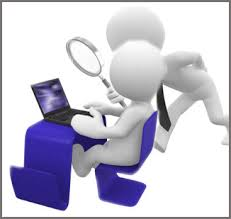
\includegraphics[scale=0.2]{Images/testing.jpeg}
		Functional tests consist in testing all the functionalities of an application.
	\end{figure}
The company has a quite big application and they have some code that they didn't develop. So we had to do a lot of functionnal tests to know all
the bugs of the application. 
As an example I can give : when we used the school bag service and we click on the button new Folder and click on the close button. Then we couldn't
click again on the new Folder button. \\
I also had to test more complicated services such as the coherence between 
teacher, parents and students accounts. For example if a teacher add
an homework for a class, all the sudents should see it as well as their parents. \\
But doing some tests without writing anything about them is not very useful for the future of the company. That's why I test all the services of the application and report about all the functionalities of every services on a 
document test. I learnt how to write lisable tests documents that is not so obvious.  

\subsection{Acceptance testing}
Individual software modules are combined and tested as a group. The purpose
of these tests is to verify functional, performance and reliability requirements. 

\subsection{Regression testing}



\subsection{JMeter}
\begin{figure}[h]
	
\includegraphics[scale=0.5]{Images/JMeter.jpeg}
	JMeter is a software to test web application.
\end{figure}


